\documentclass[a4paper,12pt,twoside,openany]{report}
%
% Wzorzec pracy dyplomowej
% J. Starzynski (jstar@iem.pw.edu.pl) na podstawie pracy dyplomowej
% mgr. inż. Błażeja Wincenciaka
% Wersja 0.1 - 8 października 2016
%
\usepackage{polski}
\usepackage{helvet}
\usepackage[T1]{fontenc}
\usepackage{anyfontsize}
\usepackage[utf8]{inputenc}
\usepackage[pdftex]{graphicx}
\usepackage{tabularx}
\usepackage{array}
\usepackage[polish]{babel}
\usepackage{subfigure}
\usepackage{amsfonts}
\usepackage{verbatim}
\usepackage{indentfirst}
\usepackage[pdftex]{hyperref}


% rozmaite polecenia pomocnicze
% gdzie rysunki?
\newcommand{\ImgPath}{.}

% oznaczenie rzeczy do zrobienia/poprawienia
\newcommand{\TODO}{\textbf{TODO}}


% wyroznienie slow kluczowych
\newcommand{\tech}{\texttt}

% na oprawe (1.0cm - 0.7cm)*2 = 0.6cm
% na oprawe (1.1cm - 0.7cm)*2 = 0.8cm
%  oddsidemargin lewy margines na nieparzystych stronach
% evensidemargin lewy margines na parzystych stronach
\def\oprawa{1.05cm}
\addtolength{\oddsidemargin}{\oprawa}
\addtolength{\evensidemargin}{-\oprawa}

% table span multirows
\usepackage{multirow}
\usepackage{enumitem}	% enumitem.pdf
\setlist{listparindent=\parindent, parsep=\parskip} % potrzebuje enumitem

%%%%%%%%%%%%%%% Dodatkowe Pakiety %%%%%%%%%%%%%%%%%
\usepackage{prmag2017}   % definiuje komendy opieku,nrindeksu, rodzaj pracy, ...


%%%%%%%%%%%%%%% Strona Tytułowa %%%%%%%%%%%%%%%%%
% To trzeba wypelnic swoimi danymi
\title{Poprawa rozdzielczości zdjęć przy użyciu krzyżowo-skalowej korelacji cech}

% autor
\author{Aliaksandr Karolik}
\nrindeksu{295138}

% jeśli wykonawca jest tylko jeden, to usuwamy poniższe polecenia
%\authorII{Pracowity Kolega}
%\nrindeksuII{654321}

\opiekun{dr inż. Grzegorz Sarwas}
%\konsultant{prof. Dzielny Konsultant}  % opcjonalnie
\terminwykonania{1 lutego 2017} % data na oświadczeniu o samodzielności
\rok{2017}


% Podziekowanie - opcjonalne
%\podziekowania{\input{podziekowania.tex}}

% To sa domyslne wartosci
% - mozna je zmienic, jesli praca jest pisana gdzie indziej niz w ZETiIS
% - mozna je wyrzucic jesli praca jest pisana w ZETiIS
\miasto{Warszawa}
\uczelnia{POLITECHNIKA WARSZAWSKA}
\wydzial{WYDZIAŁ ELEKTRYCZNY}
\instytut{INSTYTUT STEROWANIA I ELEKTRONIKI PRZEMYSŁOWEJ}
\zaklad{ZAKŁAD STEROWANIA}
\kierunekstudiow{INFORMATYKA STOSOWANA}

% domyslnie praca jest inzynierska, ale po odkomentowaniu ponizszej linii zrobi sie magisterska
%\pracamagisterska
%%% koniec od P.W



\streszczenia{
	\input{streszczenia.tex}
}

\begin{document}
\maketitle

%-----------------
% Wstęp
%-----------------
\chapter{Wstęp}
	W dobie dużej popularności cyfrowej rejestracji obrazów przy wykorzystaniu urządzeń mobilnych takich jak kamery, czy tablety za pomocą wbudowanych w  nich aparatów fotograficznych jakość/rozdzielczość zarejestrowanych obrazów nie zawsze jest zadowalająca. Zarejestrowane materiały są w różnoraki sposób zakłócone, zniekształcone, co nie pozwala nam na wydruk, w odpowiedniej jakości, tego typu materiału. Ponieważ optyka zainstalowana w średniej półki telefonach komórkowych nie pozwala na uzyskanie wystarczającej jakości fotografii, widać wyraźne zapotrzebowanie na algorytmy poprawiające rozdzielczość i jakość zarejestrowanych obrazów.
	
	Czym jest super-rozdzielczość? Super-rozdzielczość (pisana również jako super resolution, superresolution) jest określeniem zestawu metod zwiększania skali wideo lub obrazów. Terminy takie jak „skalowanie w górę”, „powiększanie”, „konwersja w górę” i „uprez” również opisują wzrost rozdzielczości w przetwarzaniu obrazu lub edycji wideo. 
	
	Większość technik super-rozdzielczości opiera się na tym samym pomyśle: wykorzystanie informacji z kilku różnych obrazów do stworzenia jednego powiększonego obrazu. Algorytmy próbują wyodrębnić szczegóły z każdego obrazu w sekwencji, aby zrekonstruować inne ramki. Obraz w wysokiej rozdzielczości oferuje dużą gęstość pikseli, a tym samym więcej szczegółów na temat oryginalnej sceny.

	Potrzeba wysokiej rozdzielczości jest powszechna w wizji komputerowej dla lepszej wydajności w rozpoznawaniu wzorów i analizie obrazów. Wysoka rozdzielczość ma znaczenie w obrazowaniu medycznym dla diagnozy. Wiele aplikacji wymaga powiększenia określonego obszaru w którym niezbędna jest wysoka rozdzielczość, np. aplikacje do nadzoru, kryminalistyki i obrazowania satelitarnego.

	Praca ta skupiać się będzie na badaniu rozwiązań algorytmicznych w dziedzinie widzenia komputerowego służących do poprawy rozdzielczości, zwanych również algorytmami super-rozdzielczości (super-resolution). 


\chapter{Algorytmy do poprawy rozdzielczości zdjęć}
W tym rozdziale opisane zostaną podstawowe, jak i obecnie używane architektury sieci neuronowych  do poprawy rozdzielczości zdjęć. Przedstawione zostaną teoretyczne podstawy działania oraz główne założenia budowy. Architektury sieci są tak dobrane, aby móc zaprezentować rozwój pomysłów ich twórców.

%-----------------
% Wstęp teoretyczny
%-----------------

\section{Wstęp teoretyczny}
	Super-rozdzielczość (SR) odnosi się do zadania przywracania obrazów o wysokiej rozdzielczości z jednej lub więcej obserwacji tej samej sceny w niskiej rozdzielczości (LR). Zgodnie z liczbą wejściowych obrazów LR, SR można podzielić na super-rozdzielczość pojedynczego obrazu (SISR) i super-rozdzielczość wielu obrazów (MISR). W porównaniu z MISR SISR jest znacznie bardziej popularną metodą ze względu na wysoką wydajność. Typowa struktura SISR jest zaprezentowana na rysunku \ref{szkicSisr}.
	\begin{figure}[!htbp]
		\begin{center}
			\centering
			\includegraphics[scale=0.3]{\ImgPath/rys/sisr.png}
		\end{center}
		\caption{Szkic SISR}
		\label{szkicSisr}
	\end{figure}
  	\newpage
  	Głównie algorytmy SISR dzielą się na trzy kategorie: metody oparte na interpolacji, metody oparte na rekonstrukcji oraz metody oparte na uczeniu. Metody SISR oparte na interpolacji, takie jak interpolacja dwusześcienna (bicubic interpolation) i próbkowanie Lanczosa (Lanczos resampling), są bardzo szybkie i proste, ale dość niedokładne.
  	  
  	Metody SR oparte na rekonstrukcji,  często przyjmują zaawansowaną wcześniejszą wiedzę w celu ograniczenia możliwej przestrzeni rozwiązań z korzyścią polegającą na generowaniu elastycznych i ostrych szczegółów. Jednak wydajność wielu metod opartych na rekonstrukcji szybko spada, gdy zwiększa się skala, oraz metody te są zwykle czasochłonne.
  
  	Metody SISR oparte na uczeniu, znane również jako metody oparte na przykładach, najczęściej używane ze względu na ich szybkie obliczenia i wyjątkową wydajność. Metody te zwykle wykorzystują algorytmy uczenia maszynowego do analizy związków statystycznych między LR i odpowiadającym mu odpowiednikiem HR z istotnych przykładów szkoleniowych.
  
  	Technika MISR wykorzystuję jako wejście zestaw obrazów niskiej rozdzielczości do budowy obrazu HR, ale jak już wcześniej było wspomniane, SISR jest popularniejsza ze względu na wysoką wydajność.

%-----------------
% Konwolucyjna sieć neuronowa
%-----------------  
  
\section{Konwolucyjna sieć neuronowa}
	Konwolucyjne sieci neuronowe (CNN) są prawie wszędzie. Jest to prawdopodobnie najbardziej popularna architektura głębokiego uczenia. Niedawny wzrost zainteresowania głębokim uczeniem wynika z ogromnej popularności i skuteczności konwulsyjnych sieci neuronowych. Zainteresowanie CNN rozpoczęło się od AlexNet \cite{NIPS2012_c399862d} w 2012 roku i od tego czasu rosło wykładniczo. W ciągu zaledwie trzech lat naukowcy przeszli z 8-warstwowej sieci AlexNet \cite{NIPS2012_c399862d} do 152-warstwowej sieci ResNet \cite{ResNet}.

	CNN jest obecnie modelem go-to dla każdego problemu związanego z obrazem. CNN również stosowane w systemach rekomendacji, przetwarzania języka naturalnego i nie tylko. Główną zaletą sieci CNN w porównaniu z jej poprzednikami jest to, że automatycznie wykrywa ona ważne cechy bez żadnego nadzoru człowieka. Na przykład, biorąc pod uwagę wiele zdjęć kotów i psów, sieć sama uczy się cech charakterystycznych dla każdej klasy.

	Podstawowym narzędziem sieci jest warstwa konwolucyjna. Warstwa konwolucyjna składa się z zestawu filtrów, zadaniem, której jest wykrycie poszczególnych cech ze zdjęcia.

	Mnożenie splotowe lub konwolucja to operacja matematyczna polegająca na połączeniu dwóch zestawów informacji. W naszym przypadku konwolucja jest stosowana na danych wejściowych oraz filtru. W wyniku powstaje nowa macierz, która jest nazywana mapą cech, wartości mapy są wynikiem kombinacji liniowej poszczególnych pikseli obrazu wejściowego i przesuwającego się filtra. Poniżej na rysunku \ref{schematKonwolucji} zaprezentowany jest schemat mnożenia splotowego lub konwolucji:
	\begin{figure}[!htbp]
		\begin{center}
			\centering
			\includegraphics[scale=0.4]{\ImgPath/rys/CNN-konwolucja-1.png}
		\end{center}
		\caption{Schemat mnożenia splotowego (konwolucji)}
		\label{schematKonwolucji}
	\end{figure}

	Tak samo, jak w zwykłej sieci, po warstwie konwolucyjnej występuje warstwa aktywacji (najczęściej używana jest funkcja ReLU), zadaniem, której jest wprowadzenie nieliniowości do sieci.
	
	Drugim podstawowym elementem sieci konwolucyjnej jest warstwa łączącą (pooling layer). Zadaniem jej jest zmniejszenie wymiarów mapy cech, wyznaczonej w warstwie konwolucyjnej, przy zachowaniu jej kluczowych elementów. Warstwa ta również odpowiada za redukcję szumu. Najczęściej używaną metodą jest „Max pooling”.

	Algorytm działania metody Max pooling jest następujący: definiowany jest filtr oraz krok przesunięcia. Kolejne wartości macierzy wyjściowej są maksymalną wartością objętą filtrem. Na rysunku \ref{schematMaxPooling} zaprezentowany jest schemat działania metody Max pooling:

	\begin{figure}[!htbp]
		\begin{center}
			\centering
			\includegraphics[scale=0.4]{\ImgPath/rys/max-pooling.png}
		\end{center}
		\caption{Schemat metody Max pooling}
		\label{schematMaxPooling}
	\end{figure}

%-----------------
% Podstawowa architektura SISR
%-----------------
\section{Konwolucyjne sieci neuronowe dla super-rodzielczości}
	Pierwszą zaproponowaną architekturę używającą CNN do mapowania obrazów niskiej rozdzielczości do wysokiej jest SRCNN \cite{SRCNN}. Architekturę SRCNN zaprezentowana jest na rysunku \ref{archSRCNN}. SRCNN jest trójwarstwowym CNN, poszczególne warstwy której składają się z filtrów o wymiarach $64 \times 1 \times 9 \times 9$, $1 \times 32 \times 5 \times 5$ i $1 \times 32 \times 5 \times 5$.
	Każda warstwa odpowiada za następujące czynności:
	\begin{enumerate}
		\item Wyodrębnienie i reprezentacja. Obraz jest przepuszczany przez zestaw filtrów. Zadaniem, których jest wyodrębnienie cech specyficznych.  
		\item Mapowanie nieliniowe. Dla każdej mapy cech wyprodukowanych w poprzedniej warstwie przyporządkowywany jest wektor cech o wysokiej rozdzielczości.
		\item Rekonstrukcja. Ostatnia warstwa konwulacyjna układa wektory cech uzyskane w poprzedniej warstwie w jeden obraz wysokiej rozdzielczości.
	\end{enumerate}
	\begin{figure}[!htbp]
		\begin{center}
			\centering
			\includegraphics[scale=0.2]{\ImgPath/rys/SRCNN.png}
		\end{center}
		\caption{Architektura SRCNN}
		\label{archSRCNN}
	\end{figure}
	
	Autorzy proponujące architekturę SRCNN przewidywali, że zwiększenie ilości warstw konwulocyjnych korzystnie wpłynie na wyniki. Niedługo po ich publikacji zaczęły pojawiać się rozwiązania o głębszych architekturach. Kim i in. zaproponowali bardzo głęboki model VDSR z ponad 16 warstwami konwolucyjnymi korzystającymi ze skutecznego uczenia rezydualnego (resztkowego,residual learning). Aby w pełni wykorzystać moc głębokich CNN, Lim i in. zintegrowali bloki rezydualne w framework SR, w wyniku powstały modeli EDSR i MDSR.

  %-----------------
  % Model CSNL
  %-----------------
\section{Model CSNLN}
	\label{ModelCSNLN}
	Modeli do poprawy rozdzielczości pojedynczego obrazu oparte na dużej ilości warstw konwolucyjcnych wykorzystują korzyści płynące z dużych zewnętrznych zasobów obrazu do lokalnej odbudowy, jednak w większości istniejących prac pominięto dalekosiężne podobieństwa cech charakterystycznych. Niektóre z ostatnich prac z powodzeniem wykorzystały te wewnętrzne korelacje cech, używając nielokalne moduły uwagi.
	
	Jednakże istniejące podejścia do odtwarzania obrazów używały jedynie podobieństwa cech w tej samej skali, ignorując liczne wewnętrzne wzorce LR-HR w różnych skalach, co prowadziło do stosunkowo niskiej wydajności. Wiadomo, że wewnętrzne korelacje HR zawierają bardziej istotne informacje o wysokich częstotliwościach. W tym celu,  Yiqun Mei i in. w swoim artykule \cite{CSNLN} proponują pierwszy moduł uwagi Cross-Scale Non-Local (CS-NL) z integracją do rekurencyjnej sieci neuronowej. 
	
	Proponowana architektura sieci przedstawiona jest na rysunku \ref{CSNLN}. Jest to w zasadzie rekurencyjna sieć neuronowa, w której każda komórka zwana Self-Exemplars Mining (SEM) w pełni integruje uczenie oparte o lokalne czynniki, nielokalne czynniki w tej samej skali obrazów oraz w skali zmiennej używając nowo proponowany moduł CS-NL.
	
	Powtarzające się komórki SEM są osadzone w sekwencyjną strukturę, jak pokazano na rysunku \ref{CSNLN}. Każda komórka SEM produkuje $H_i$ przekształconą mapę cech powstającą z połączenia wyników dwóch modułów uwagi oraz mapy cech otrzymanej ze zwykłej warstwy konwolucyjnej. Wydobyte mapy cech $H_i$ łączone jedną warstwą konwulacyjną w wyniku łączenia powstaje obraz wysokiej rozdzielczości.
	
	\begin{figure}[!htbp]
		\begin{center}
			\centering
			\includegraphics[scale=0.6]{\ImgPath/rys/CSNLN.png}
		\end{center}
		\caption{Architektura CSNLN}
		\label{CSNLN}
	\end{figure}
	\subsection{Moduły uwagi}
	
	Jak było już wspomniano wcześniej wybrany algorytm wyszukuje nielokalne korelacje w obrazach w tej samej skali oraz w skali zmiennej. Korelacje poszukiwane są za pomocą dwóch modułów uwagi nielokalnej o nazwach  In-Scale Non-Local Attention (IS-NL) oraz Cross-Scale Non-Local Attention (CS-NL).
	
	Nielokalna uwaga może eksplorować próbki poprzez podsumowanie cech charakterystycznych ze zbioru obrazów wejściowych. Autorzy publikacji używająć artykułu \cite{NonLocalAttention} zdefiniowali nielokalną uwagę dla wybranej $X$ mapy cech obrazu przy pomocy wzoru \ref{nonlocalAtten}.
	
	\begin{equation}
		Z_{i,j}= \sum_{g,h}\frac{\exp (\phi(X_{i,j},X_{g,h}))}{\sum_{u,v}\exp(\phi(X_{i,j},X_{u,v}))} \psi(X_{g,h}),
		\label{nonlocalAtten}
	\end{equation}
	gdzie: 
	\begin{itemize}
		\item $(i,j),(g,h)$ oraz $(u,v)$ pary kordynat mapy $X$
		\item $\phi(.)$ funkcja transformacji cech
		\item $\psi(.,.)$ funkcją korelacji do pomiaru podobieństwa. Definiowana w sposób \ref{kor}
	\end{itemize}
	\begin{equation}
		\psi(X_{i,j},X_{g,h}) = \theta(X_{i,j})^T \delta(X_{g,h}),
		\label{kor}
	\end{equation}
	gdzie: 
	\begin{itemize}
		\item $\theta(.), \delta(.)$ funkcje transformacji cech
	\end{itemize}

	W oparciu o wzór \ref{nonlocalAtten} autorzy zaimplementowali moduł IS-NL poniżej na rysunku \ref{IS-NL} jest graficzna reprezentacja.
	
	\begin{figure}[!htbp]
		\begin{center}
			\centering
			\includegraphics[scale=1.2]{\ImgPath/rys/Attention.png}
		\end{center}
		\caption{Moduł IS-NL}
		\label{IS-NL}
	\end{figure}

	Powyższe sformułowanie \ref{nonlocalAtten} zostało rozszerzone do wersji używającej krzyżowo-skalową korelację cech. Zamiast pomiaru wzajemnej korelacji pikselowej jak jest robione w modułu IS-NL, proponowany nowy moduł uwagi ma na celu pomiar korelacji pomiędzy pikselami o niskiej rozdzielczości a plastrami większej skali obrazu LR.
	% DO poprawy
	
	Na rysunku \ref{CS-NL} zaprezentowana została architektura modułu uwagi wykorzystująca krzyżowo-skalową korelację cech zaprojektowana w oparciu o \ref{nonlocalAtten} przez twórców artykułu. Moduł CS-NL działa w następujący sposób wejściowa mapa cech $X$ o wymiarach $W \times H$ przekształcana jest przy pomocy interpolacji dwuliniowej do $Y$ o wymiarach $\frac{W}{s} \times \frac{H}{s}$. Następnie plastry $p \times p$ z mapy $X$ są porównywany do $p \times p$ w mapie $Y$ aby uzyskać wynik dopasowania softmax. Na samym końcu jest używana warstwa dekonwolucyjna na wynikach softmaxa oraz wagach plastra o wymiarze $sp \times sp$ wydobywana z mapy $X$. W wyniku powstaje mapa Z o wymiarach $sW \times sH$, która będzie $s$ razy bardziej określona niż $X$.
	
	\begin{figure}[!htbp]
		\begin{center}
			\centering
			\includegraphics[scale=0.5]{\ImgPath/rys/CS-NL.png}
		\end{center}
		\caption{Moduł CS-NL}
		\label{CS-NL}
	\end{figure} 


	%Autorzy zaporoponowali następujący algorytm do pomiaru krzyżowo-skalowej korelacji cech. Aby wyszukać podobieństwo piksela do plastra skala wejściowej mapy cech $X$ o wymiarach $W \times H$ zostaje obniżona o $s$ czyli powstaje $Y$ o wymiarach $\frac{W}{s} \times \frac{H}{s}$. Wyszukiwane jest pikselowe podobieństwo $X$ z $Y$ oraz używjąc odpowiadający plaster o wymiarach $s \times s$ z mapy $X$ do stworzenia pixeli o wększej rozdzielczości. W wyniku tych operacji powstanie mapa cech o wymiarach $sW \times sH$. Poniżej jest zaprezentowany zadoptowany wzór do wyszukiwania krzyżowo skalowej korelacji cehc.
	%\begin{equation}
	%	Z_{si,sj}^{s\times s}= \sum_{g,h}\frac{\exp (\phi(X_{i,j},Y_{g,h}))}{\sum_{u,v}\exp(\phi(X_{i,j},Y_{u,v}))} \psi(X_{sg,sh}^{s\times s}),
	%	\label{nonlocalAtten}
	%\end{equation}
	\subsection{Mutual-Projected Fusion}
	Jak wcześniej było wspomniane, każda komórka SEM zawiera trójbranżową strukturę, przy pomocy której generuje trzy mapy cech poprzez niezależne wykorzystanie każdego ze źródeł informacji z obrazów LR, niejasne pozostaje, jak połączyć te oddzielne tensory w kompleksową mapę funkcji. Autorzy zaproponowali własny algorytm do stopniowego łączenia cech. Procedura algorytmu została przedstawiona na rysunku \ref{Fusion}.
	
	Aby pozwolić sieci skupić się na bardziej informacyjnych cechach najpierw jest obliczana różnica $R_{IC}$ pomiędzy dwoma mapami cech $F_I$ i $F_C$ z modułów IS-NL oraz CS-NL odpowiednio. Następnie wynikowa mapa $R_{IC}$ jest przepuszczana przez jedną warstwę konwolucyjną, później z powrotem jest dodawana mapa $F_I$ jest to robione do przewrócenia straconych informacji przy operacji odejmowania.
	\begin{equation}
		R_{IC}  = F_I - F_C
		\label{RIC}
	\end{equation}
	\begin{equation}
		F_{IC} = conv(R_{IC}) + F_I
 		\label{FIC}
	\end{equation}
	Pozostająca cecha $R_{IC}$ reprezentuje szczegóły istniejące w jednym źródle, a brakujące w drugim. Taka projekcja pozwala sieci skupić się tylko na odrębnych informacjach pomiędzy źródłami, omijając przy tym powszechną wiedzę, co zwiększa jej zdolność dyskryminacyjną.
	\begin{figure}[!htbp]
		\begin{center}
			\centering
			\includegraphics[scale=0.5]{\ImgPath/rys/fusion.png}
		\end{center}
		\caption{Algorytm lączenia map cech}
		\label{Fusion}
	\end{figure} 
	
	Wzorując się artykułem DBPN \cite{DBPN}, autorzy zaadoptowali podejście back-projection w celu włączenia lokalnych informacji, aby dodać regularyzację cech i skorygować błędy rekonstrukcji. Wynikowa mapa $H$ jest obliczana w następujący sposób. 
	\begin{equation}
		e = F_L - downsample(F_{IC}),
		\label{RIC}
	\end{equation}
	\begin{equation}
		H = upsample(e) + F_{IC}
		\label{FIC}
	\end{equation}
	gdzie $F_L$ jest mapą cech z gałęzi lokalnej (Local branch), $downsample$ jest dokonywany przy pomocy warstwy konwolucyjnej do zmniejszenia wymiaru oraz $upsample$ odpowiednio warstwa konwolucyjna do przewrócenia wymiarów do $sH \times sW$.
	
	Zaproponowany algorytm gwarantuje uczenie resztkowe (residual learning) przy jednoczesnym łączeniu różnych źródeł cech, co umożliwia bardziej dyskryminacyjne uczenie w porównaniu do zwykłego dodawania lub łączenia.
\newpage
\section{Model EDSR}
	Aby zweryfikować skuteczność modelu CSNLN, postanowiono porównać otrzymane wyniki do metody state-of-the-art o nazwie EDSR \cite{EDSR} (ang. Enhanced Deep Residual Networks for Single Image Super-Resolution). Wybór takiego modelu był podyktowany częstym odwoływaniem się do wspomnianego modelu w wielu artykułach naukowych napotkanych w trakcie przeglądania literatury związanej z dziedziną problemu.
	
	Architektura modelu EDSR zaprezentowany na  rysunku \ref{EDSR}. Struktura modelu jest podobna do sieci SRResNet \cite{SRResNet}, ale zaproponowany model nie posiada warstw aktywacji poza blokami rezydualnymi. Dodatkowo w modelu EDSR zostały  zmodyfikowane bloki rezydualne. 
	
		\begin{figure}[!htbp]
		\begin{center}
			\centering
			\includegraphics[scale=0.5]{\ImgPath/rys/EDSR_Architecture.png}
		\end{center}
		\caption{Architektura modelu EDSR}
		\label{EDSR}
	\end{figure} 
	\newpage
	Rysunku \ref{EDSR_resBlok} zawiera nowo proponowany blok rezydualny wraz z porównaniem go z blokiem z sieci ResNet oraz SRResNet. Nowo proponowany blok składa się tylko z dwóch warstw konwolucyjnych oraz warstwy aktywacji. Jak widać z rysunku \ref{EDSR_resBlok} warstwy normalizacji wsadowej (ang. Batch Normalization) zostały usunięte. Taka decyzja była podjęta, ponieważ warstwy normalizacji wsadowej, pozbywają się elastyczności sieci poprzez normalizację cech obrazu wejściowego.
	
	Taka konfiguracja modelu bez warstwy normalizacji pozwoliła zaoszczędzić około 40\% zużycia pamięci podczas szkolenia, w porównaniu z SRResNet \cite{SRResNet}.
	\begin{figure}[!htbp]
		\begin{center}
			\centering
			\includegraphics[scale=0.6]{\ImgPath/rys/EDSRresudualbloc.png}
		\end{center}
		\caption{Architektura modelu EDSR}
		\label{EDSR_resBlok}
	\end{figure}
	  %-----------------
  % Stegoanaliza
  %-----------------
  %\newpage

\chapter{Implementacje}
	W tym rozdziale zostaną przedstawione implementacje wcześniej opisanego modelu oraz benchmarku do poprawy rozdzielczości zdjęć. Modeli były przygotowywane do rozwiązania problemu dwukrotnego oraz trzechkrotnego powiększania rozdzielczości zaszumionych obrazów.

\section{Środowisko programistyczne}
	Rozpoczynając pracę nad modelami, używany był własny komputer Lenovo Yoga 500 z kartą graficzną Nvidia Geforce 940M oraz systemem operacyjnym Linux 20.04.1 LTS. Po przeanalizowaniu implementacji wybranych metod stało się jasne, że nie uda się przeprowadzić proces uczenia na własnej maszynie ze względu na zbyt małą ilość pamięci graficznej. Rozwiązaniem tego problemu było udostępnienie mnie karty graficznej \textbf{Nvidia Geforce RTX 2080} na serwerze politechniki warszawskiej. Lokalne środowisko zostało przeniesione  na serwer.

	Język programowania został wybrany \textbf{Python}. Ze względu na wcześniejszą znajomość języka, duży zbiór narzędzi do wizualizacji i przekształcania obrazów oraz ogromną popularność w zastosowaniach związanych ze sztuczną inteligencją.

	Jako biblioteka do uczenia maszynowego została wybrana \textbf{PyTorch}. Głównie wybór był spowodowany istniejącymi implementacjami modeli oraz chęcią poznania tej biblioteki jako narzędzia, które będzie używane w przyszłości.

	Do tworzenia własnych datasetów wykorzystano biblioteki \textbf{Pillow} i \textbf{OpenCV}. Są to zaawansowane biblioteki języka programowania Python, udostępniające zestawy modułów służących do obróbki grafiki.


\section{Zbiory danych}
\label{Zbior danych}
%% tu musi być ref do zbioru danych w bibliografii
	Do uczenia modeli zostało wykorystano trzy zbiory danych:
	\begin{enumerate}
		\item zbiór  danych DIV2K,
		\item własny zbiór danych zawierający tylko  zaszumione obrazy,
		\item własny zbiór danych zawierający obrazy zaszumione jak i nie zaszumione.
	\end{enumerate}
	
	Pierwszym zbiorem danych był zbiór o nazwie \textbf{DIV2K} \cite{DIV2K}. Jest to zbiór 1000 kolorowych obrazów RGB, autorzy tworzące ten zbiór zwracali szczególną uwagę na jakość obrazu, różnorodność źródeł (stron i kamer). Obrazy niskiej rozdzielczości uzyskiwane przez pomniejszenie zdjęć ze zbioru za pomocą interpolacji dwusześciennej. Zbiór był używany do wyzwań NTIRE (2017, 2018) oraz PIRM 2018. Zbiór DIV2K składa się:
	\begin{itemize}
		\item zbioru uczącego. Zbiór zawiera 800 par obrazów  o  wysokiej  i nizkiej  rozdzielczości.
		\item zbioru validacyjnego.  Zbiór zawiera 100 par obrazów  o  wysokiej  i nizkiej  rozdzielczości.
		\item zbioru testowego. Zbiór zawiera 100 par obrazów  o  wysokiej  i nizkiej  rozdzielczości.
	\end{itemize}

	Biorąc pod uwagę jakość obrazów zbioru DIV2K ze stanem faktycznym zdjęć robionych przy pomocy telefonu komórkowego, postanowiono stworzyć własne zbiory danych. Do tego wybrano 150 obrazów, zrobionych za pomocą własnego telefonu komórkowego Huawei P20 rozdzielczość obrazów wynosiła $4160 \times 3120$. Zbiór zawierał zdjęcia natury, ludzi, krajobrazów oraz zwierząt.

	Drugi zbiór danych wykorzystywany do trenowania i walidacji modeli został utworzony wykorzystując wcześniej opisane zdjęcia. Tworzony on był z myślą o sprawdzenie jak modeli będą radzić z zadaniem odszumiania zdjęć. Aby to sprawdzić każde zdjęcie zostało zinterpolowano za pomocą interpolacji dwuliniowej oraz po zmniejszeniu każdy obraz był powielony czterokrotnie z dodaniem różnych szumów. W tym przypadku zostały wykorzystane następujące szumy:
	\begin{itemize}
		\item szum Gausowski,
		\item szum Gausowski z lokalne odchylenia w każdym punkcie obrazu,
		\item szum typu sół,
		\item szum typu piepsz.
	\end{itemize} 

	Ostatni zbiór danych wejściowych był zrobiony jako kombinacja zdjęć zaszumionych i zinterpolowanych. Taki zbiór zapewniał dużą zdolność generalizacji, bo w przypadku modeli uczonych tylko na zdjęciach zaszumionych nie były one w stanie zapewnić dobrą jakość obrazu w przypadku gdy na wejście trafiały obrazy niezaszumione. 

	Podstawowy zbiór zawierający 150 obrazów był powielany pięciokrotnie. Każde zdjęcie również było poddawane interpolacji dwuliniowej, ale tylko dwa zdjęcia z pięciu były poddawane zaszumieniu. Pozostałe trzy zdjęcia były niezmieniane. Używane były następujące szumy:
	\begin{itemize}
	 	\item szum Gausowski,
	 	\item połączenie szumów sół i piepsz.
	\end{itemize} 

\section{Model CSNLN}
\label{Model CSNLN}
	Pracując nad przygotowaniem modeli CSNLN do poprawy rozdzielczości zdjęć, wykorzystano artykuł \cite{CSNLN} z 2020 roku oraz oficjalną implementację autorów artykułu, która jest ogólnie dostępna na GitHub. Zastosowano architekturę przedstawioną w tej publikacji, która była  wcześniej opisana  w  sekcji  \ref{ModelCSNLN}. Model składał się z 12 komórek SEM. W każdej z warstw modelu używano funkcji aktywacji ReLU. Wykres tej funkcji jest zaprezentowany na rysunku \ref{relu}.
	\begin{figure}[!htbp]
		\begin{center}
			\centering
			\includegraphics[scale=0.3]{\ImgPath/rys/relu.png}
		\end{center}
		\caption{Wykres funkcji ReLU}
		\label{relu}
	\end{figure}    

	Model był trenowany przy pomocy normy $L^1$, jednak była podjęta próba udoskonalenie modelu przez zmianę funkcji strat na $L^2$. Do optymalizacji wag modeli użyto algorytmu Adam o współczynnikach $\beta_1=0.9$, $\beta_2=0.999$ oraz $\epsilon=1e-8$. 
	
	Zgonie z publikacją rozmiar wejściowy obrazów (ang. patch) wynosił $48 \times 48$, jednak został on zmniejszony do $34 \times 34$ dla dwukrotnego oraz $36 \times 36$ trzechkrotnego powiększenia. Wybór takich był uwarunkowany dostępnej ilością pamięci graficznej. Ewaluacja modeli następowała po przerobieniu 16 zdjęć (ang. batch). Początkowy krok uczenia wynosił $1e-4$.
	
	Rysunek \ref{CSNLN_uczenie} przedstawia wykresy uczenia oraz ewaluacji modeli. 
	\begin{figure}[!htbp]
		
		\begin{center}
			\centering
			\subfigure[Trenowanie ]{\includegraphics[scale=0.4]{\ImgPath/rys/CSNLNtrain_loss_L1.pdf}}
			\subfigure[Walidacja]{\includegraphics[scale=0.4]{\ImgPath/rys/CSNLNtest_loss_L1.pdf}}
		\end{center}
		\caption{Wykresy funkcji strat w procesie uczenia modelu CSNLN}
		\label{CSNLN_uczenie}
	\end{figure}


\section{Model EDSR}
\label{Model_EDSR}
Badania zostały wykonane na podstawie oficjalnej implementacji, która jest ogólnie dostępna na GitHub. Kod został zaktualizowany do najnowszych dostępnych bibliotek na podstawie artykułu \cite{EDSR}. Konfiguracja obrazów wejściowych była zostawiona taka sama jak w przypadku modelu CSNLN opisanego w sekcji \ref{Model CSNLN}.

Zgodnie z artykułem zostały wykorzystane 32 bloki rezydualne oraz liczba kanałów była ustawiona na 256. Podczas treningu sieci, do optymalizacji jej parametrów wykorzystano algorytm Adam o współczynniku zdefiniowanych w artykule, czyli $\beta_1=0.9$, $\beta_2=0.999$ oraz $\epsilon=1e-8$. Jako funkcję straty przyjęto normę $L^1$. Początkowy krok uczenia był ustawiony $1e-4$. Ewaluacja modelu odbywała się po przejściu 16 obrazów.

Przebieg uczenia oraz ewaluacji modeli zaprezentowano na Rysunku \ref{EDSR_uczenie}.
\begin{figure}[!htbp]	
	\begin{center}
		\centering
		\subfigure[Trenowanie ]{\includegraphics[scale=0.4]{\ImgPath/rys/EDSRtrain_loss_L1.pdf}}
		\subfigure[Walidacja]{\includegraphics[scale=0.4]{\ImgPath/rys/EDSRtest_loss_L1.pdf}}
	\end{center}
	\caption{Wykresy funkcji strat w procesie uczenia modelu EDSR}
	\label{EDSR_uczenie}
\end{figure}

\section{Metryki porównania jakości modeli}
Do porównania wyników działania algorytóm zostały wykorzystane następujące metryki:
\begin{itemize}
	\item Szczytowy stosunek sygnału do szumu (PSNR, ang. peak signal-to-noise ratio)
	\item Podobieństwo strukturalne (SSIM, ang. structure similarity) 
\end{itemize}
\subsection{Szczytowy stosunek sygnału do szumu}
Szczytowy stosunek sygnału do szumu, rzadziej nazywany jako stosunek sygnału szczytowego do szumu (PSNR, ang. peak signal-to-noise ratio) – stosunek maksymalnej mocy sygnału do mocy szumu zakłócającego ten sygnał. Ze względu na szeroki zakres wartości PSNR wyrażany jest w decybelach. 

Najczęściej PSNR stosowany jest do oceny jakości kodeków wykorzystujących stratną kompresję obrazów. W takim przypadku sygnałem są nieskompresowane dane źródłowe, a szumem – artefakty (zniekształcenia) spowodowane zastosowaniem kompresji stratnej.

W celu wyznaczenia PSNR należy najpierw obliczyć współczynnik MSE (ang. mean squared error) bazujący na obu porównywanych obrazach, wykorzystując wzór \ref{MSE}. A później używając współczynik MSE obliczyć szczytowy stosunek sygnału do szumu za pomocą wzoru \ref{PSNR}. 

\begin{equation}
	MSE= \frac{1}{M*N} \sum_{i=1}^{N} \sum_{j=1}^{M} ([f(i,j)-f'(i,j)]^2) \label{MSE}
\end{equation}

Gdzie:
\begin{itemize}
	\item $N,M$ - wymiary obrazu w pikselach,
	\item $f(i,j)$- wartość piksela o współrzędnych $(i,j)$ obrzu oryginalnego,
	\item $f'(i,j)$- wartość piksela o wpółrzędnych $(i,j)$ obrazu skompresowanego.
\end{itemize}

\begin{equation}
	PSNR= 10 log_{10}{\frac{[max(f(i,j))]^2}{MSE}}
	\label{PSNR}
\end{equation}
Gdzie: 
\begin{itemize}
	\item $max(f(i,j))$ – wartość maksymalna danego sygnału; w przypadku obrazów zwykle jest to wartość stała, np. dla obrazów monochromatycznych o reprezentacji 8-bitowej wynosi $255$.
\end{itemize}

\subsection{Podobieństwo strukturalne}
Podobieństwo strukturalne ( SSIM ) jest metodą przewidywania postrzeganej jakości telewizji cyfrowej i obrazów filmowych, a także innych rodzajów zdjęć i filmów cyfrowych. Indeks SSIM jest metodą pełnego porównania, innymi słowy, mierzy jakość w oparciu o oryginalny obraz (nie skompresowany lub bez zniekształceń). Wskaźnik SSIM jest rozwinięciem tradycyjnych metod, takich jak PSNR (peak signal-to-noise ratio) i standardowej metody średniego błędu kwadratowego (MSE), które okazały się niezgodne z fizjologią ludzkiego postrzegania. 

Indeks SSIM zawiera się w przedziale od $-1$ do $+1$. Wartość $+1$ jest osiągana tylko wtedy, gdy próbki są w pełni autentyczne. Indeks SSIM jest obliczany w różnych oknach obrazu. Miara pomiędzy dwoma oknami $x$ i $y$ o wspólnym rozmiarze $N \times N$ obliczana jest za pomocą wzoru \ref{SSIM}. 

\begin{equation}
	SSIM(x,y)= \frac{(2\mu_x\mu_y+c_1)(2\sigma_{xy}+c_2)}{(\mu_x^2+\mu_y^2+c_1)(\sigma_x^2+\sigma_y^2+c_2)}
	\label{SSIM}
\end{equation}

Gdzie: 
\begin{itemize}
	\item $\mu_x$ wartość średnia z $x$
	\item $\mu_y$ wartość średnia z $y$
	\item $\sigma_x^2$ wariancja $x$
	\item $\sigma_y^2$ wariancja $y$
	\item $\sigma_{xy}$ kowariancja $x$ i $y$
	\item $c_1=(k_1L)^2, c_2=(k_2L)^2$ dwie zmienne stabilizujące podział ze słabym mianownikiem
	\item $L$ zakres dynamiki wartości pikseli 
	\item $k_1=0.01$ i $k_2=0.03$
\end{itemize}
\chapter{Testowanie wybranych  modeli}
	W tym rozdziale zostały zaprezentowane oraz opisane wyniki przeprowadzonych badań wytrenowanych modelach na pierwszym zbiorze danych opisanym w sekcji \ref{Zbior danych}. Zamieszczone zostały metryki porównawcze działania algorytmów dla zdjęć pomniejszonych. Również znajdzie się w tym rozdziale porównanie rozmiarów wytrenowanych modeli dla dwukrotnego oraz trzechkrotnego powiększenia obrazu.

\section{Testowanie na zbiorze danych DIV2K}  
\label{TestDIV2K}
	W pierwszej części testów postanowiono sprawdzenie wyników modelu przedstawione w publikacji. Jednak proces uczenia nie był dokładnie powtórzony, jak opisuje artykuł. Proces trenowania był przerywany po przejściu 100 epok oraz, jak już było wspomniane, wejściowe obrazy miały mniejsze wymiary.
	
	W tablice \ref{TabelaDIV2k} są zaprezentowane uzyskane wyniki na zbiorze testowym Set5 \cite{Set5}. Również tabela \ref{TabelaDIV2k} zawiera wyniki powiększenia obrazów przy pomocy interpolacji. Decyzja zamieszczenia tych wyników była kierowana chęcią pokazania efektów działania najprostszych metod powiększenia obrazów w porównaniu do głębokich sieci neuronowych.
	
	\begin{table}[!htbp] 
		\centering
	\begin{tabular}{ |p{5cm}||p{2cm}|p{2cm}|p{2cm}|  }
		\hline
		Algorytm & Skala & PSNR &SSIM \\
		\hline
		Interpolacja dwuliniowa                   & x2   &30.422&  0.901\\
		Interpolacja dwusześcienna                & x2   &32.399&   0.928\\
		EDSR                                      &   x2   & 35.841&   0.943\\
		CSNLN  ($L^1$)  						  &   x2  & 36.026& 0.955\\
		CSNLN ($L^2$)  							  &   x2  & 35.721& 0.933\\
		\hline
		Interpolacja dwuliniowa                   &   x3  &26.396&   0.808\\
		Interpolacja dwusześcienna                &   x3  & 26.913   &0.825\\
		EDSR                                      &   x3 & 32.532 &  0.903\\
		CSNLN ($L^1$) 						      &   x3  & 33.169 & 0.932\\
		CSNLN ($L^2$)  							  &   x3  & 32.321 & 0.912\\
		\hline
		
	\end{tabular}
	\caption{Wyniki metod uzyskane na zbiorze testowym}
	\label{TabelaDIV2k}
	\end{table}
	
	Wśród interpolacji wyniki są tym lepsze, im złożonej jest metoda interpolacji. Jak i było przewidywano, wyniki uzyskane przy pomocy sieci neuronowych są lepsze w stosunku do interpolacji. Jednak różnią się oni od wyników pokazanych w publikacji, chociaż i nie wiele. Najprawdopodobniej jest to spowodowane zmniejszeniem wymiarów wejściowych obrazu oraz krótszym czasem trenowania. 
	
	Drugim czynnikiem wpłynącym na uzyskane wartości metryk mogła być zmiana przestrzeni barw, na podstawie której były pozyskiwane wartości PSNR i SSIM. W publikacji PSNR i SSIM obliczane dla składowej Y w przestrzeni barw YCbCr natomiast wartości pokazane w tabeli \ref{TabelaDIV2k} były obliczane w przestrzeni RGB.
	
	Na rysunku \ref{fig:DIv2k} zaprezentowane zostały wyniki powiększenia zdjęcia ze zbioru testowego Set5 \cite{Set5}. Wyniki ilustrują działanie dwóch wariantów interpolacji oraz dwóch głębokich sieci neuronowych.
	
	\begin{figure}[!htbp]
		\centering
		\subfigure[Set5 (x2):  baby.png]{\includegraphics[width=0.45\textwidth]{\ImgPath/rys/testy/DIV2k/babyShowReactangle.png}}
		\subfigure[HR]{\includegraphics[width=0.25\textwidth]{\ImgPath/rys/testy/DIV2k/babyCrop.png}} 
		\subfigure[Interpolacja dwuliniowa]{\includegraphics[width=0.25\textwidth]{\ImgPath/rys/testy/DIV2k/Bilenierbaby_x2_SRCrop.png}} 
		\subfigure[Interpolacja dwusześcienna]{\includegraphics[width=0.27\textwidth]{\ImgPath/rys/testy/DIV2k/baby_x2_SRCropBicubic.png}}
		\subfigure[EDSR]{\includegraphics[width=0.27\textwidth]{\ImgPath/rys/testy/DIV2k/EDSRbabyCrop_x2.png}}
		\subfigure[CSNLN]{\includegraphics[width=0.27\textwidth]{\ImgPath/rys/testy/DIV2k/CSNLNbabyCrop_x2.png}}
		\caption{Porównanie wizualne dla skali  x2 na zbiorze danych Set5}
		\label{fig:DIv2k}
	\end{figure}
	
	Zdecydowanie najgorszy wynik był uzyskany przy użyciu interpolacji dwuliniowej, zdjęcie jest bardzo rozmyte. Nieco lepiej wygląda zdjęcie uzyskane przy pomocy interpolacji dwusześciennej, kolory wyglądają bardzo naturalnie. Punkty, w których występują skupienia takich samych pikseli, są mniej rozmyte. Jednak wynik uzyskany przy pomocy interpolacji jest nie do zaakceptowania, ponieważ nadal rozmycie jest zauważalne.
	
	Znacznie lepiej prezentują się wyniki uzyskane przy pomocy głębokich sieci neuronowych. Pod względem ostrości obie sieci radzą skuteczniej w porównaniu do wyników uzyskanych za pomocą interpolacji. Trudno jednak stwierdzić która sieć działa lepiej wizualnie, bo różnice widoczny tylko przy dogłębnym przejrzeniu.
	
	Tablica \ref{fig:DIv2k} zawiera wyniki próby udoskonalenie modelu przez zmianę funkcji strat na $L^2$. Eksperymenty wskazują, że trenowanie z użyciem normy $L^1$ osiąga lepsze wyniki.
	\newpage
\section{Rozmiary modeli}
	W tabeli \ref{TabelaSizeOfModels} zaraportowane rozmiary modeli oraz ich skuteczność. Łatwo zauważyć, że model CSNLN jest lżejszy niż EDSR. Potrzebuje tylko 7\% rozmiaru modeli EDSR dla dwukrotnego oraz 13\% dla trzechkrotnego powiększenia. Jednak do otrzymania lepszych wyników model CSNLN ma w dwa razy dłuższy czas treningu niż EDSR. 
		\begin{table}[!htbp] 
			\centering
			\begin{tabular}{ |p{5cm}||p{1cm}|p{2cm}|p{2cm}|  }
				\hline
				& Skala & EDSR &  CSNLN \\
				\hline		
				Rozmiar modelu                            &   x2  &  43.68M    &  3.06M \\
				Czas trenowania							  &   x2  &  20 godzin &  46 godzin\\
				PSNR								      &   x2  &  35.841    &  36.026\\
				\hline
				Rozmiar modelu                            &   x3  &  43.68M    &   6.01M\\
				Czas trenowania							  &   x3  &  20 godzin &  46 godzin\\
				PSNR								      &   x3  &  32.532    &  33.169\\
				\hline
				
			\end{tabular}
			\caption{Rozmiar modelu i porównanie wydajności dla zbioru Set5}
			\label{TabelaSizeOfModels}
		\end{table}

\newpage
\chapter{Usuwanie szumu z obrazów}
W tym rozdziale zostały zaprezentowane oraz opisane wyniki przeprowadzonych badań zdolności modeli opisanych w sekcjach \ref{Model CSNLN}, \ref{Model_EDSR} usuwać szum z obrazów przy jednoczesnym ich powiększeniu.
%Zamieszczone zostały metryki porównawcze działania algorytmów  oraz odszumione zdjęcia. 
\section{Eksperement z użyciem zbioru tylko zasumionych obrazów}
  
	Eksperyment polegał na sprawdzeniu który z modeli lepiej rozwiązuję problem otrzymania zdjęć przy jednoczesnym ich powiększeniu. Wytrenowano sieci EDSR oraz CSNLN przy użyciu drugiego zbioru danych opisanego w sekcji \ref{Zbior danych}. Każdy z modeli został następnie przetestowany w działaniu na zdjęciach. Wyniki tych testów demonstruje tablica \ref{TabelaShum}.
	
	\begin{table}[!htbp] 
		\centering
		\begin{tabular}{ |p{3cm}||p{2cm}|p{2cm}|p{2cm}|  }
			\hline
			Algorytm 							      & Skala   & PSNR      & SSIM \\
			\hline
			EDSR                                      &   x2	& 31.808	& 0.845\\
			CSNLN  ($L^1$)  						  &   x2	& 31.112	& 0.832\\
			CSNLN ($L^2$)  							  &   x2	& 31.423	& 0.838\\
			\hline
			EDSR                                      &   x3	& 31.681	& 0.860\\
			CSNLN ($L^1$) 						      &   x3	& 31.453	& 0.853\\
			CSNLN ($L^2$)  							  &   x3	& 31.723	& 0.867\\
			\hline
			
		\end{tabular}
		\caption{Wyniki uzyskane na zbiorze testowym}
		\label{TabelaShum}
	\end{table}

	Dla dwukrotnego powiększenia najlepsze wyniki zostały uzyskane przy pomocy modeli EDSR. Uzyskanie takich wyników może być związane z tym, że architektura EDSR ma globalne połączenie, omijające bloki rezydualne, w wyniku sieć uczy się głównie różnicy pomiędzy zdjęciami HR i LR. Różnica pomiędzy wynikami modeli EDSR i CSNLN jest niewielka. Zmiana funkcji straty korzystnie wpłynęła na rezultaty modelu CSNLN.
	
	W przypadku trzechkrotnego powiększenia najlepsze wyniki uzyskano przy pomocy modelu CSNLN, chociaż i nie wiele lepsze niż wynik uzyskany przez model EDSR. Jak i w przypadku dwukrotnego powiększenia obrazu zmiana funkcji straty wpłynęła pozytywnie na wyniki.
	
	Na rysunku \ref{fig:cropShum} zostały umieszczone fragmenty z zasumionego obrazu wejściowego oraz wynikowymi obrazami, które udało się uzyskać. Całkowity obraz z którego został zrobiony wycinek dla rysunku \ref{fig:cropShum} jest przedstawiony na rysunku \ref{FullImage}. Z rysunku widać, że obie sieci dobrze poradzili z problemem usuwania szumu, jednak wyjściowym zdjęciom widocznie brakowało ostrości. Po przeanalizowaniu wyników stwierdzono, że problem mógł być związany z używanym zbiorem danych, modeli dostawały tylko zaszumione zdjęcia. Aby rozwiązać ten problem, został wykreowany rozszerzony zbiór danych o zdjęcia tylko pomniejszone opisany w sekcji \ref{Zbior danych}. Wyniki eksperymentów na takim zbiorze zaprezentowane zostały w sekcji \ref{SecondEksp}.
	
	\begin{figure}[!htbp]
		\centering
		\subfigure[HR]{\includegraphics[width=0.27\textwidth]{\ImgPath/rys/testy/shum/601crop.png}}
		\subfigure[LR]{\includegraphics[width=0.27\textwidth]{\ImgPath/rys/testy/shum/601x2crop.png}} 
		\subfigure[EDSR]{\includegraphics[width=0.25\textwidth]{\ImgPath/rys/testy/shum/601_x2_EDSRMSEcrop.png}}
		\subfigure[CSNLN ($L^1$)]{\includegraphics[width=0.27\textwidth]{\ImgPath/rys/testy/shum/601_x2_CSNLNL1crop.png}}
		\subfigure[CSNLN ($L^2$)]{\includegraphics[width=0.27\textwidth]{\ImgPath/rys/testy/shum/601_x2_CSNLNMSEcrop.png}}
		\caption{Porównanie wizualne wycinka ze zdjęcia}
		\label{fig:cropShum}
	\end{figure}
	\begin{figure}[!htbp]
	\begin{center}
		\centering
		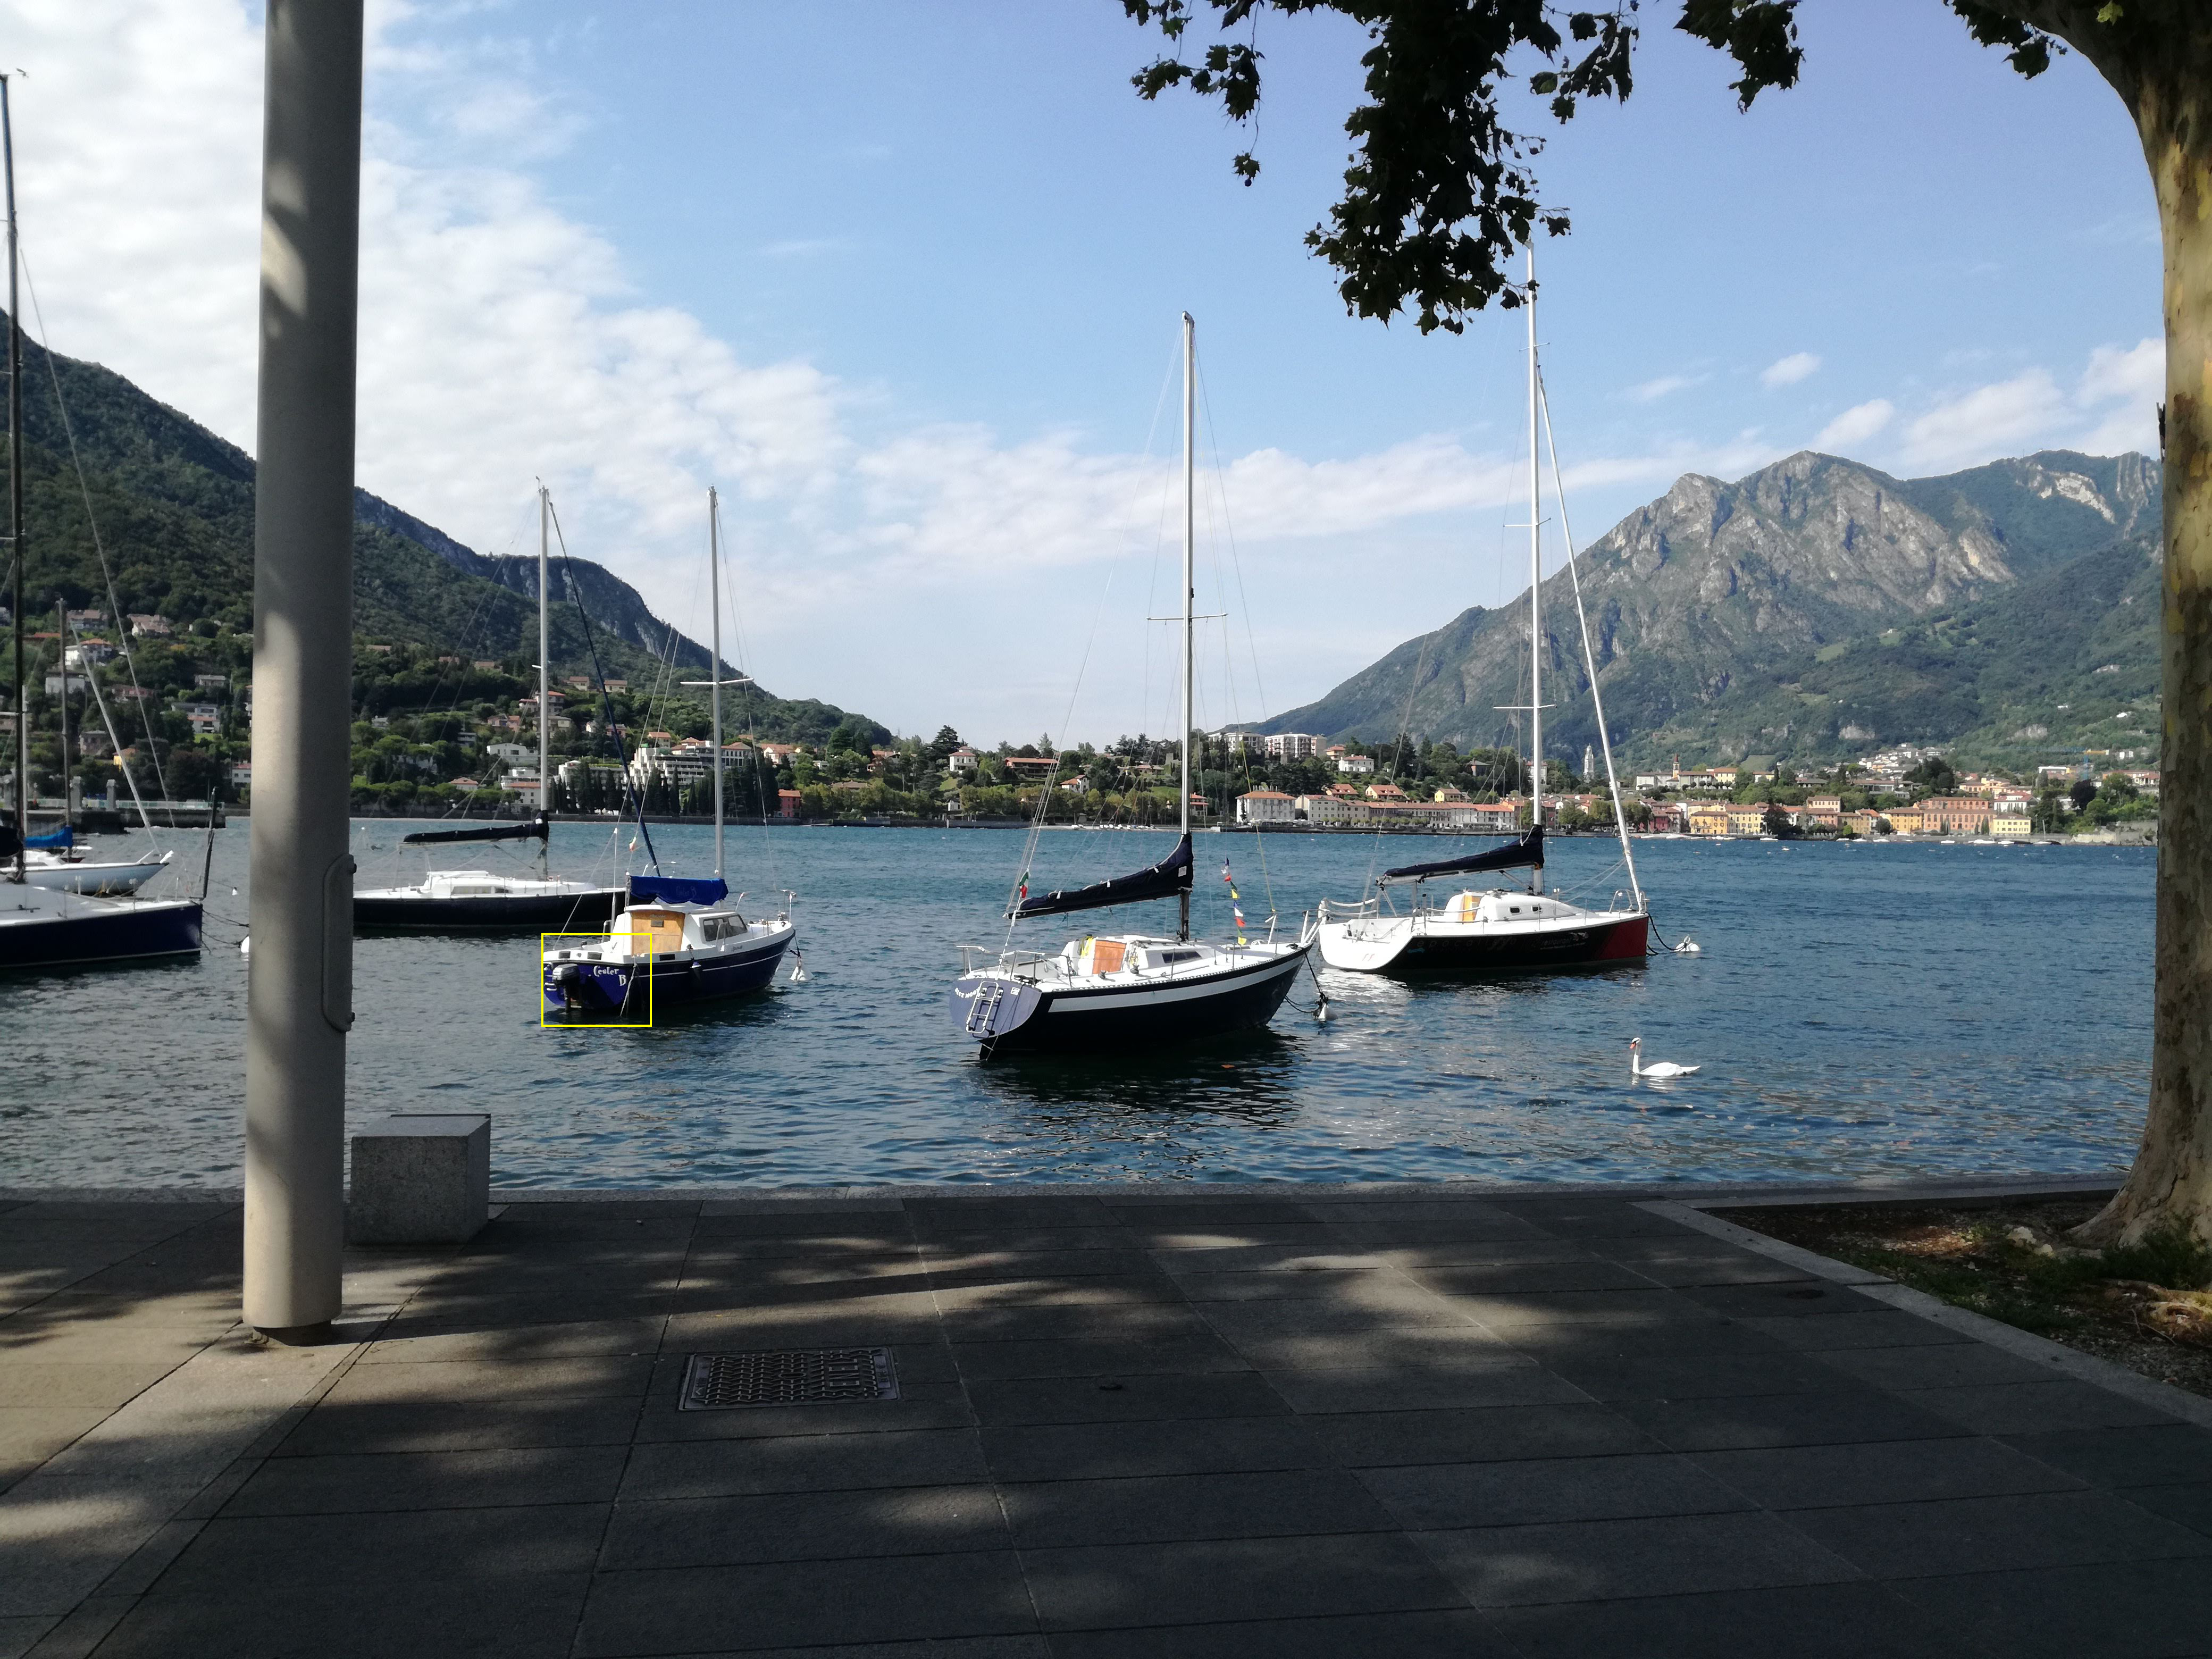
\includegraphics[width=0.8\textwidth]{\ImgPath/rys/testy/shumAndNormal/751CropReactangle.png}
	\end{center}
	\caption{Całkowity obraz testowy}
	\label{FullImage}
	\end{figure}
\newpage
\section{Eksperement z użyciem zbioru rozszerzonego}
	\label{SecondEksp}
	Celem eksperymentu było wytrenowanie modeli na zbiorze zawierającym zdjęcia zaszumione i niezaszumione. W rezultacie takiego treningu oczekiwany jest model, który będzie miał wysoką zdolność do generalizacji swojej wiedzy na nowe przypadki. Przewidywano, że model musi działać poprawnie dla zdjęć zaszumionych również, jak i niezaszumiony.
	
	Do sprawdzenia wytrenowanych modeli był użyty własny zbiór danych zawierający zdjęcia zaszumione i niezaszumione oraz wcześniej wspomniany zbiór Set5 \cite{Set5}. Wyniki uzyskane przez modeli zostały zamieszczone w tabelach \ref{TabelaShumAndNormal}, \ref{TabelaShumAndNormalSet5}.
	
	\begin{table}[!htbp] 
		\centering
		\begin{tabular}{ |p{3cm}||p{2cm}|p{2cm}|p{2cm}|  }
			\hline
			Algorytm 							      & Skala   & PSNR      & SSIM \\
			\hline
			EDSR                                      &   x2	& 34.937	& 0.918\\
			CSNLN  ($L^1$)  						  &   x2	& 34.661	& 0.916\\
			CSNLN ($L^2$)  							  &   x2	& 34.615	& 0.915\\
			\hline
			EDSR                                      &   x3	& 29.321	& 0.831\\
			CSNLN ($L^1$) 						      &   x3	& 29.418	& 0.834\\
			CSNLN ($L^2$)  							  &   x3	& 29.185	& 0.829\\
			\hline
			
		\end{tabular}
		\caption{Wyniki uzyskane na zbiorze testowym}
		\label{TabelaShumAndNormal}
	\end{table}
	\begin{table}[!htbp] 
		\centering
		\begin{tabular}{ |p{3cm}||p{2cm}|p{2cm}|p{2cm}|  }
			\hline
			Algorytm 							      & Skala   & PSNR      & SSIM \\
			\hline
			EDSR                                      &   x2	& 31.899	& 0.938\\
			CSNLN  ($L^1$)  						  &   x2	& 32.083	& 0.939\\
			CSNLN ($L^2$)  							  &   x2	& 31.997	& 0.937\\
			\hline
			EDSR                                      &   x3	& 27.478	& 0.840\\
			CSNLN ($L^1$) 						      &   x3	& 27.138	& 0.854\\
			CSNLN ($L^2$)  							  &   x3	& 27.503	& 0.858\\
			\hline
			
		\end{tabular}
		\caption{Wyniki uzyskane na zbiorze testowym Set5}
		\label{TabelaShumAndNormalSet5}
	\end{table}

	Dla dwukrotnego powiększenia zdjęć z własnego zbioru testowego najlepsze wyniki uzyskano przy pomocy modelu EDSR. W przypadku modelu CSNLN zmiana funkcji straty nie wniosła zauważalnego rezultatu. Jednak dla trzykrotnego powiększenia model CSNLN przy wykorzystywaniu normy $L^1$ osiągał najlepsze wyniki na zbiorze testowym. Jak i w przypadku dwukrotnego powiększenia zmiana funkcji straty na $L^2$ nie doprowadziła do usprawnienia działania modelu.
	\newpage
	W przypadku zbioru danych Set5 \cite{Set5} zadziwiające rezultaty pokazał model CSNLN uzyskano przez niego najlepsze rezultaty dla dwukrotnego oraz trzykrotnego powiększenia. Względem tabeli \ref{TabelaDIV2k} z sekcji \ref{TestDIV2K} wyniki uzyskane przez modeli wydają bardzo słabe, jednak trzeba mieć na uwadze to, że modeli były trenowane na zdjęciach nie idealnie wykonanych w przeciwieństwu do zbioru DIV2K \cite{DIV2K}. Najprawdopodobniej jakość zdjęć wchodzących do zbioru uczącego była powodem uzyskania aż tak niskich rezultatów na zbiorze Set5 \cite{Set5}.
	
	Na Rysunkach \ref{fig:cropShumandNormalx2}, \ref{fig:cropShumandNormalx3} zaprezentowane zostały wyniki powiększania oraz oryginał zdjęcia ze zbioru testowego. Zaprezentowany został  tylko wycinek ze zdjęcia bo nie miało sensu zamieszczenie całego obrazu ze wzgłędu na wyjściowy wymiar.
	Z obu rysunków widać potencjał oraz skuteczność stosowania głębokiego uczenia do poprawy rozdzielczości zdjęć. Jak i w przypadku modeli trenowanych na zbiorze DIV2K \cite{DIV2K} model CSNLN najlępsze wyniki uzykał dla wększej skali powiększania co jest z godne z artykułem naukowym \cite{CSNLN}.	
	\begin{figure}[!htbp]
		\centering
		%\subfigure[Całe zdjęcie HR]{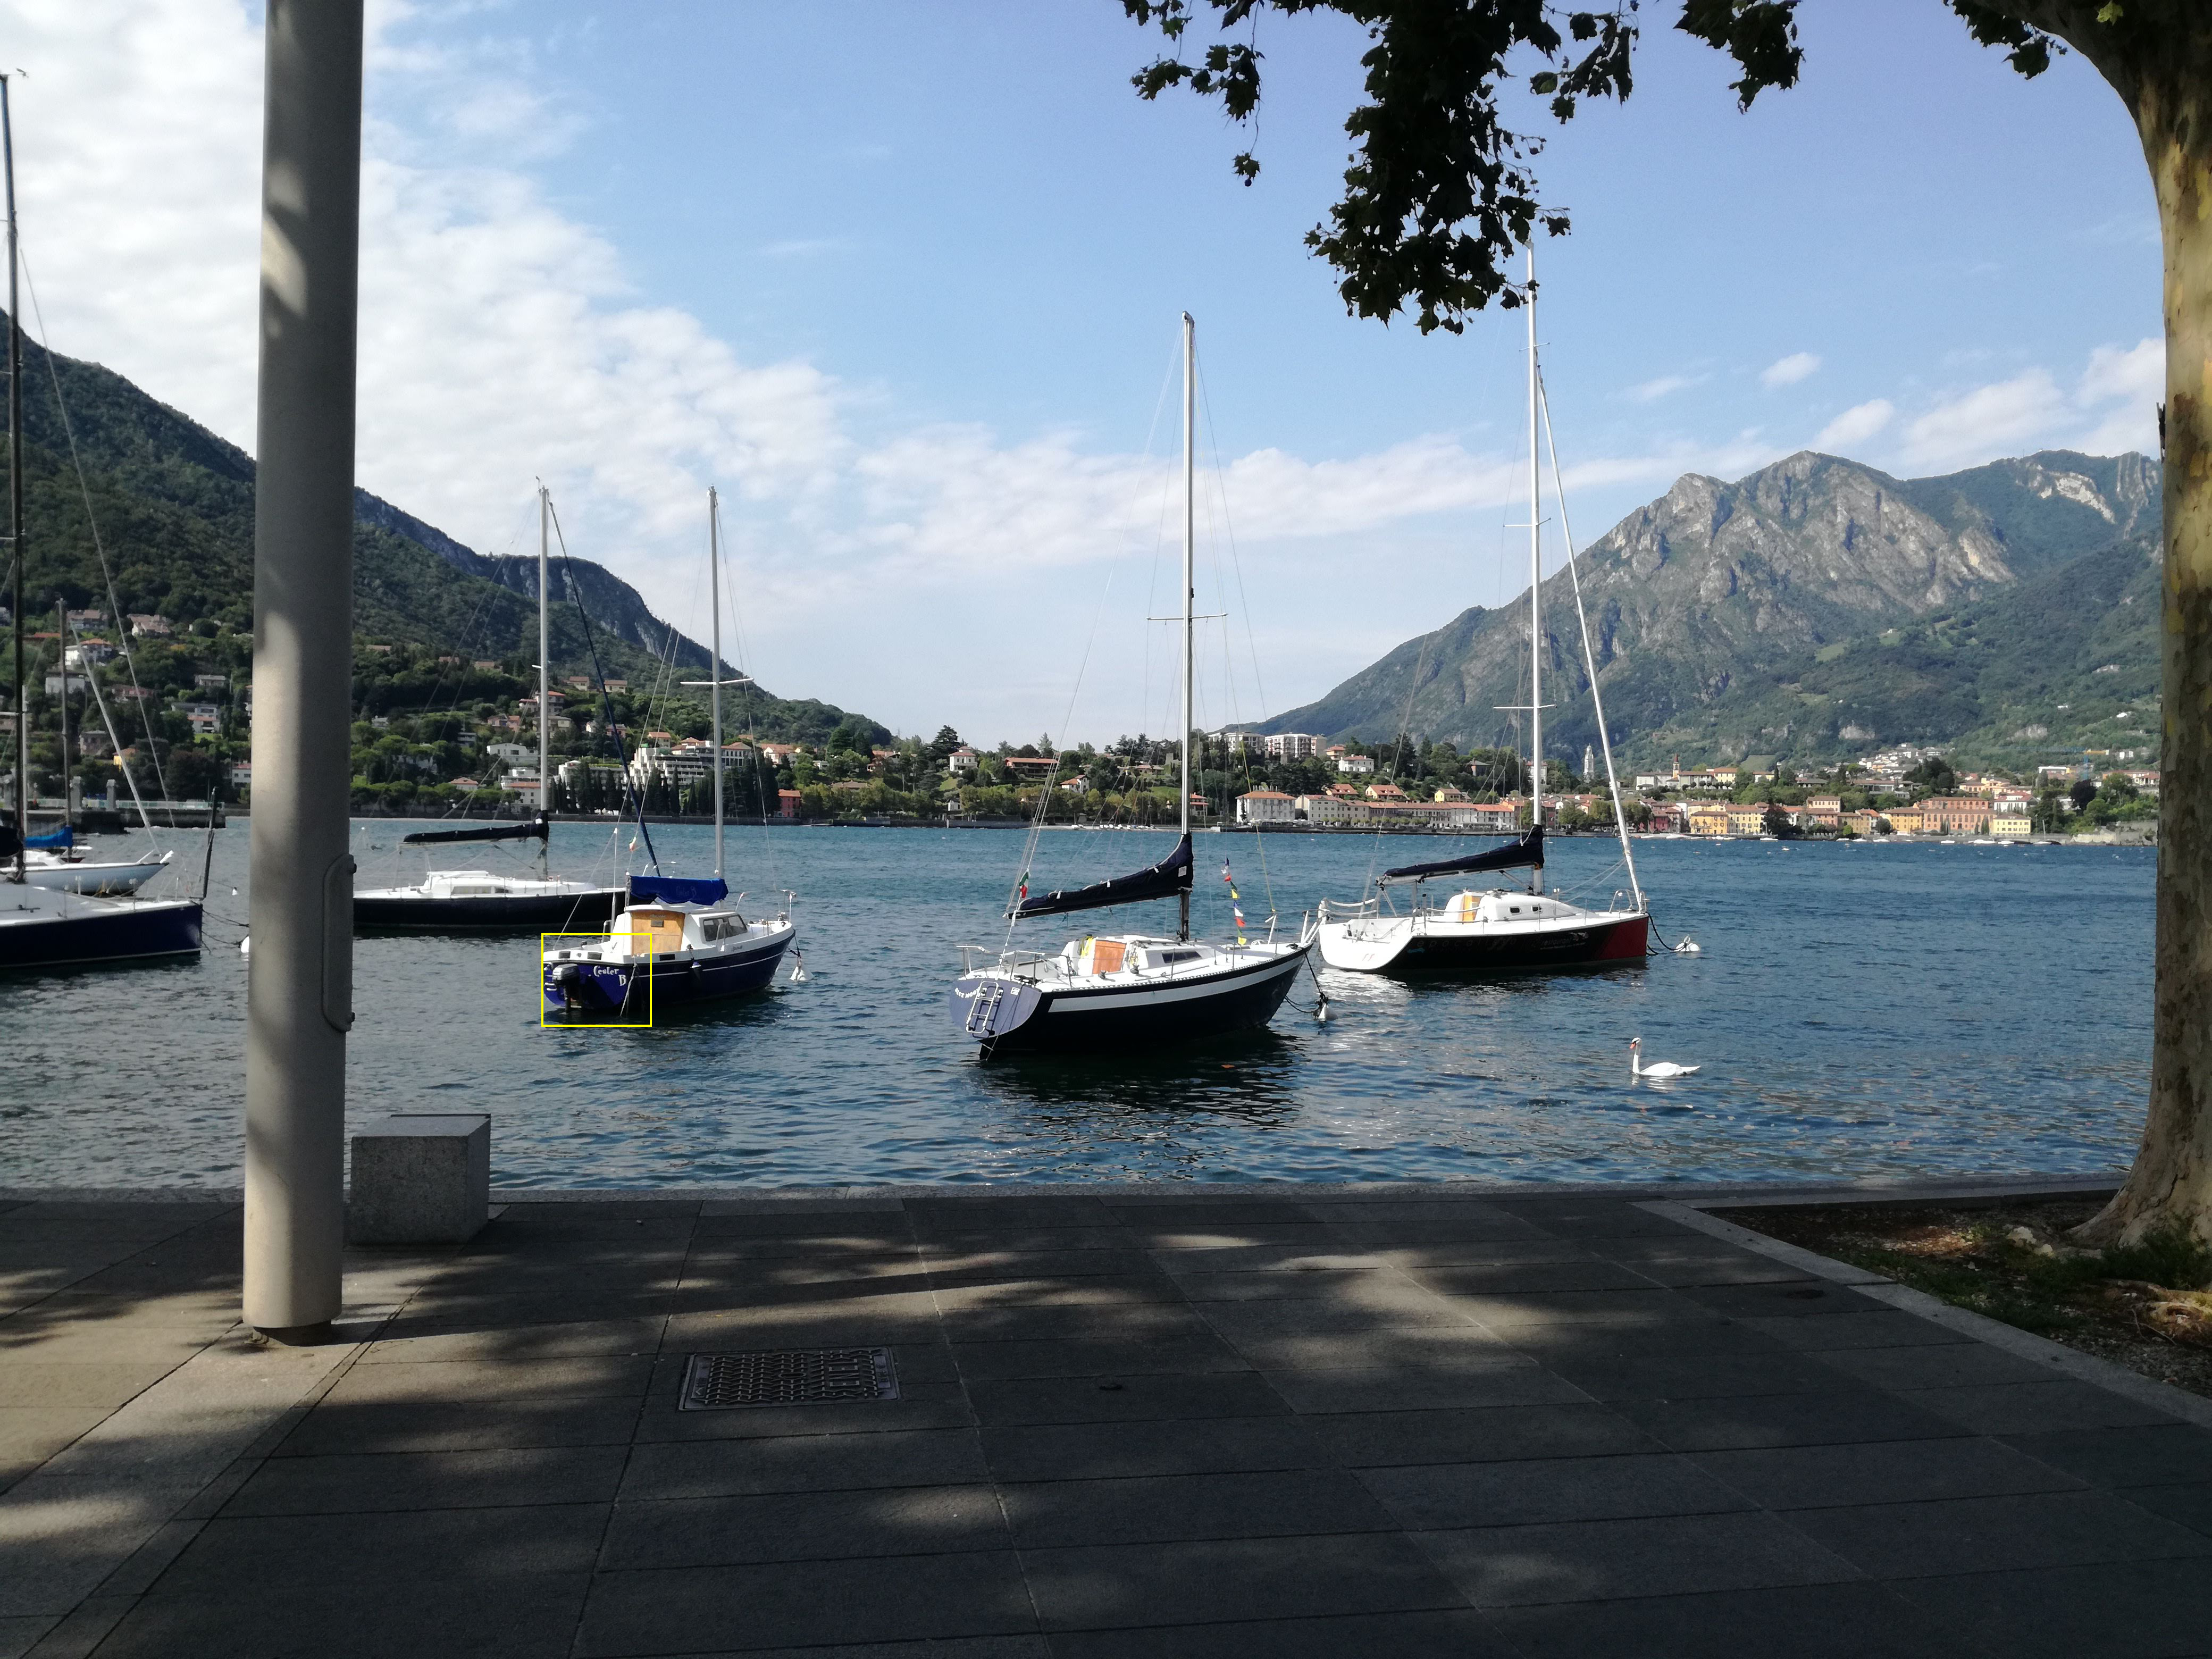
\includegraphics[width=0.27\textwidth]{\ImgPath/rys/testy/shumAndNormal/751CropReactangle.png}}
		\subfigure[HR]{\includegraphics[width=0.27\textwidth]{\ImgPath/rys/testy/shum/601crop.png}}
		\subfigure[LR]{\includegraphics[width=0.27\textwidth]{\ImgPath/rys/testy/shum/601x2crop.png}} 
		\subfigure[EDSR]{\includegraphics[width=0.27\textwidth]{\ImgPath/rys/testy/shumAndNormal/752crop_x2_SREDSR.png}}
		\subfigure[CSNLN($L^1$)]{\includegraphics[width=0.27\textwidth]{\ImgPath/rys/testy/shumAndNormal/752crop_x2_SRCSNLNL1.png}}
		\subfigure[CSNLN($L^2$)]{\includegraphics[width=0.27\textwidth]{\ImgPath/rys/testy/shumAndNormal/752crop_x2_SRCSNLNMSE.png}}
		\caption{Porównanie wizualne wycinka ze zdjęcia. Dwukrotne powiększenie.}
		\label{fig:cropShumandNormalx2}
	\end{figure}

	\begin{figure}[!htbp]
		\centering
		%\subfigure[Całe zdjęcie HR]{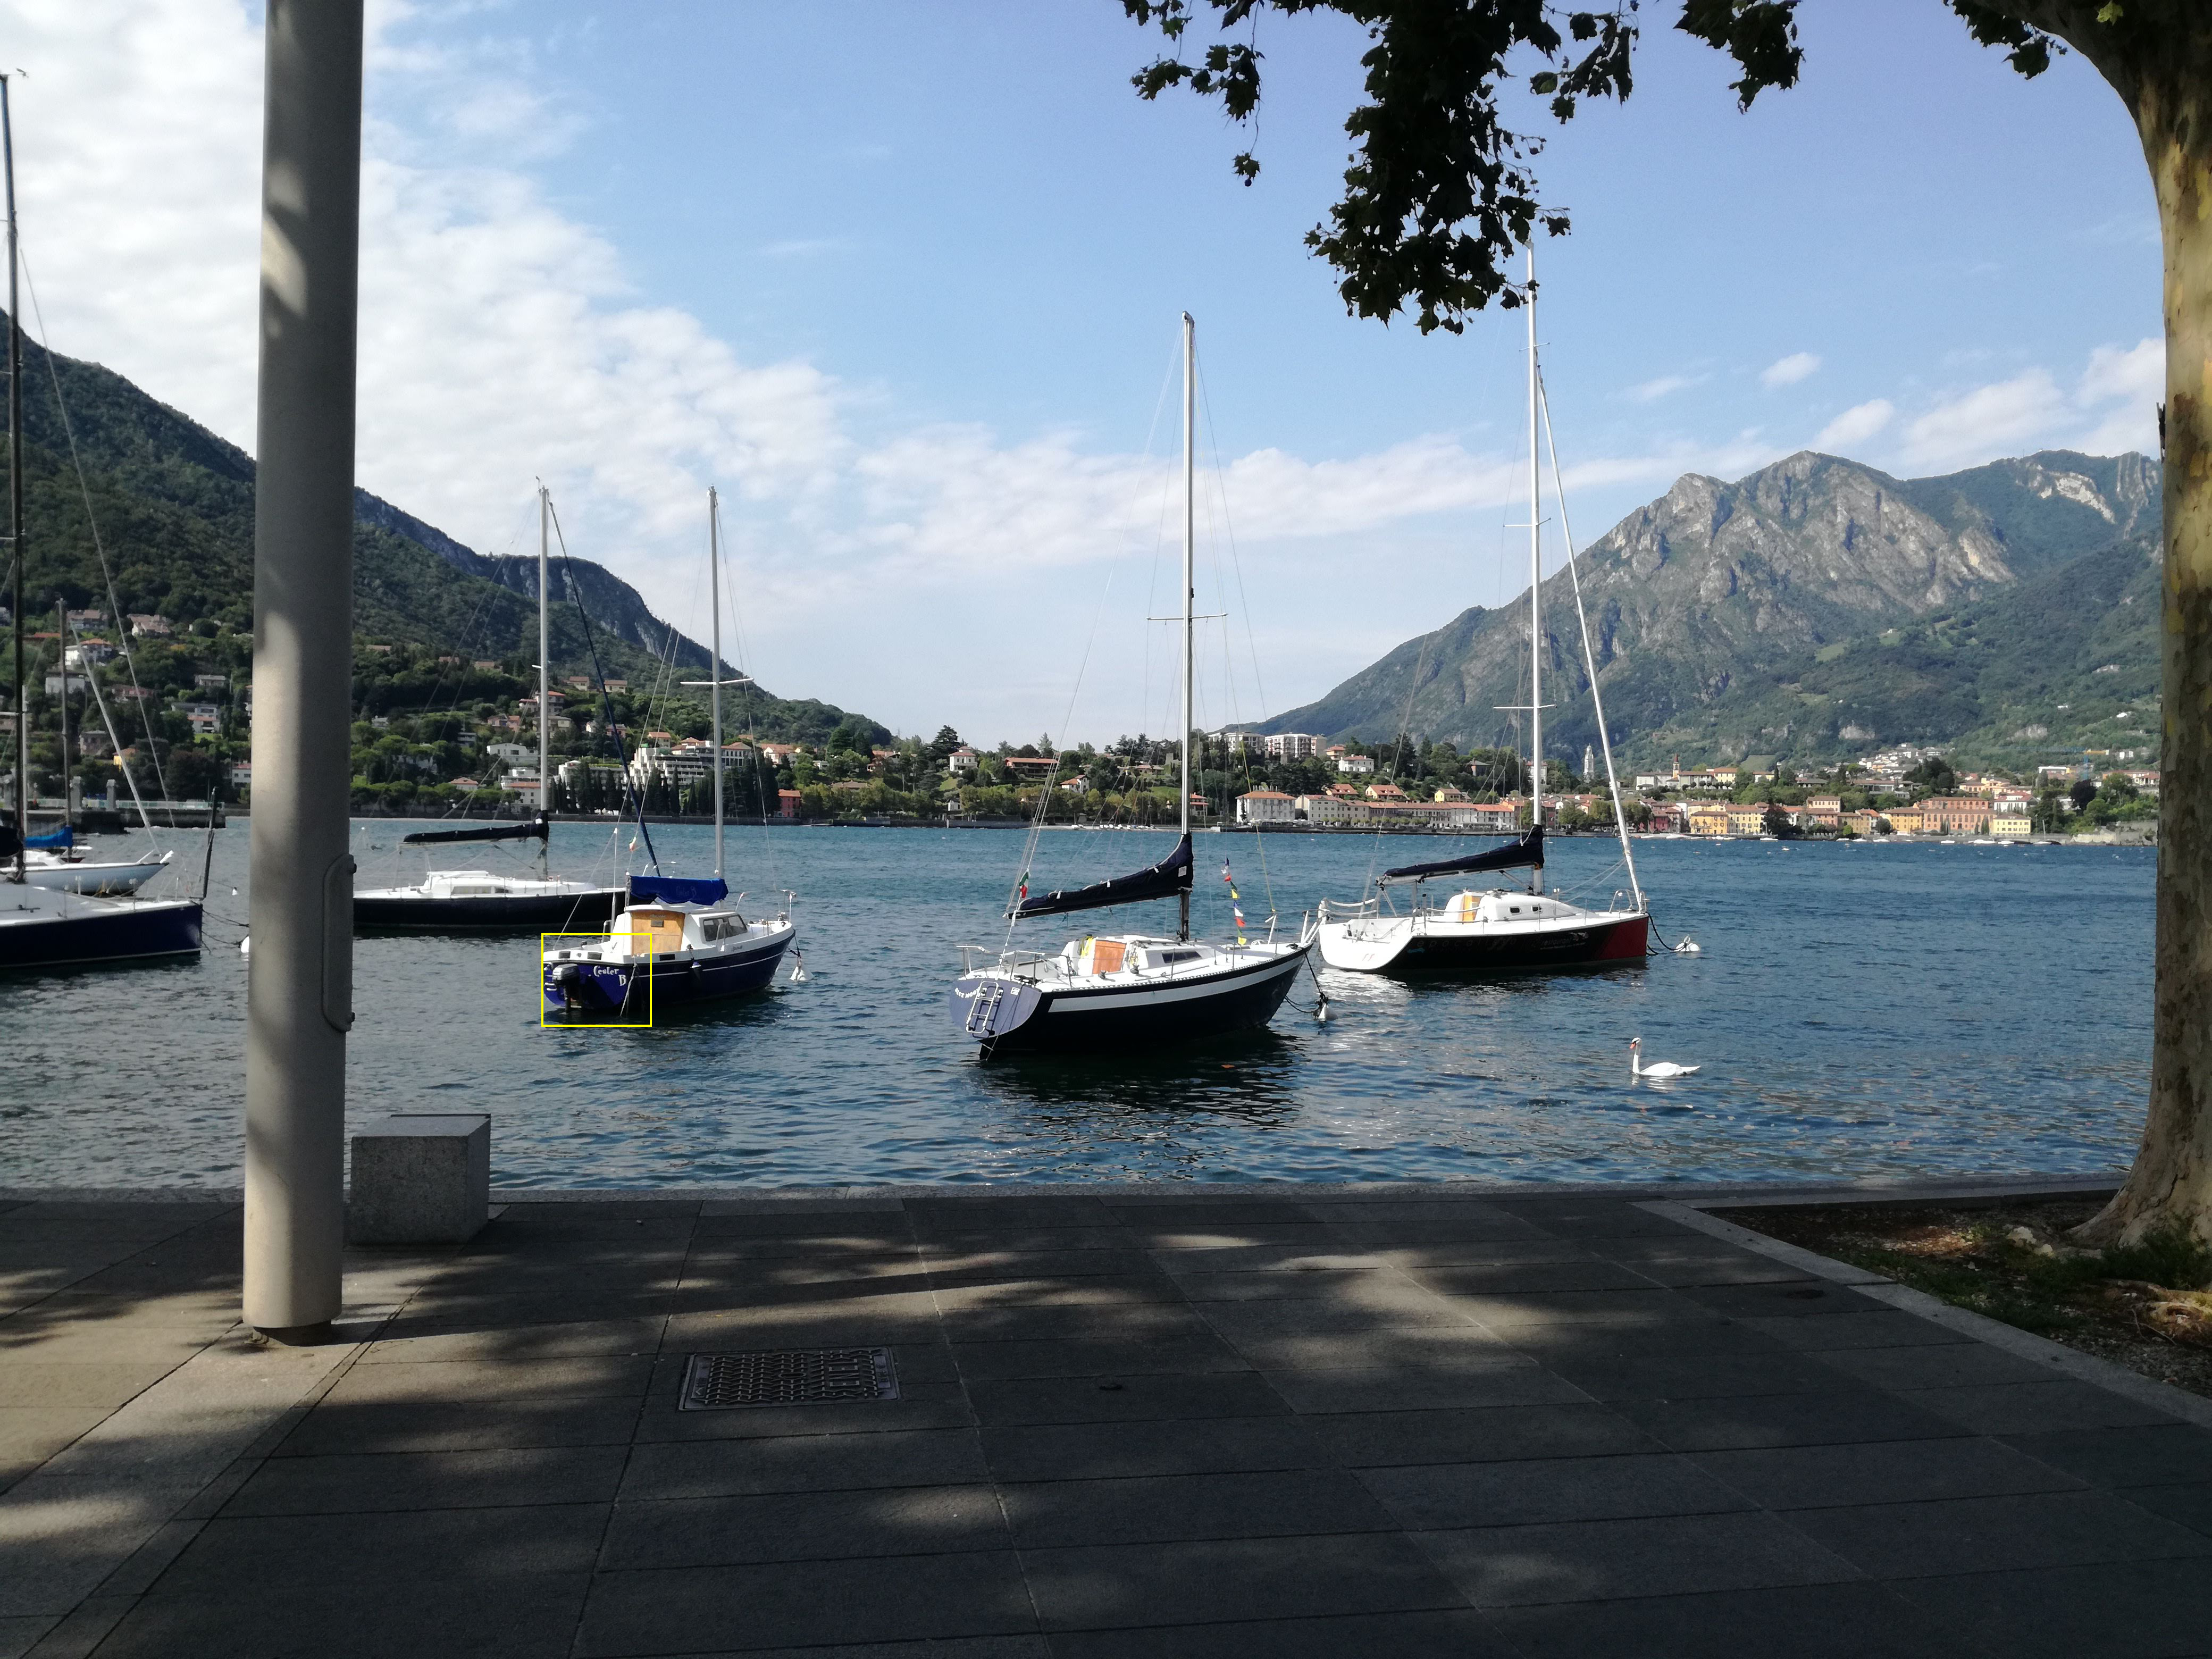
\includegraphics[width=0.27\textwidth]{\ImgPath/rys/testy/shumAndNormal/751CropReactangle.png}}
		\subfigure[HR]{\includegraphics[width=0.27\textwidth]{\ImgPath/rys/testy/shum/601crop.png}}
		\subfigure[LR]{\includegraphics[width=0.27\textwidth]{\ImgPath/rys/testy/shumAndNormal/751x3crop.png}} 
		\subfigure[EDSR]{\includegraphics[width=0.27\textwidth]{\ImgPath/rys/testy/shumAndNormal/CSNLNL1752crop_x3_SR.png}}
		\subfigure[CSNLN($L^1$)]{\includegraphics[width=0.27\textwidth]{\ImgPath/rys/testy/shumAndNormal/CSNLNL1752crop_x3_SR.png}}
		\subfigure[CSNLN($L^2$)]{\includegraphics[width=0.27\textwidth]{\ImgPath/rys/testy/shumAndNormal/CSNLNMSE752crop_x3_SR.png}}
		\caption{Porównanie wizualne wycinka ze zdjęcia. Trzykrotne powiększenie.}
		\label{fig:cropShumandNormalx3}
	\end{figure}	
	\newpage
	Założenia że rozszerzenie zbioru uczącego o zdjęcia nie zaszumione zwiększą zdolność modelu do generalizacji zostały potwierdzone. Rysunek \ref{fig:cropShumandNormal} zawiera wizualne porównanie potwierdzające korzysci wpływające z rozszerzenia zbioru uczącego. Otrzymany obraz jest bardzo wyraźny, precyzyjny  w porównaniu do obrazu otrzymanego przy pomocy modelu uczącego się tylko na zdjęciach zasumionych 
	\begin{figure}[!htbp]
		\centering
		\subfigure[CSNLN($L^1$) drugi zbiór danych]{\includegraphics[width=0.4\textwidth]{\ImgPath/rys/testy/shumAndNormal/baby_x2_SRCSRNLSHUM.png}}
		\subfigure[CSNLN($L^1$) trzeci zbiór danych ]{\includegraphics[width=0.4\textwidth]{\ImgPath/rys/testy/shumAndNormal/baby_x2_SRCSNLN.png}}
		\caption{Porównanie wizualne zdjęcia ze zbioru Set5}
		\label{fig:cropShumandNormal}
	\end{figure}
\chapter{Podsumowanie}
W pracy udało się dogłębnie przeanalizować rozwiązania służące poprawie rozdzielczości zdjęć, szczególnie to oparte na krzyżowo-skalowej korelacji cech. Cel pracy został spełniony. Zaimplementowane zostały dwa rozwiązania bazujące na sieciach splotowych – EDSR oraz CSNLN. W ostatnim z nich została wprowadzona modyfikacja w postaci zmiany funkcji aktywacji. Sieci zostały następnie przetestowane i porównane między sobą. O ile standardowe metryki jakości obrazów wygenerowanych przez sieci były podobne do zamieszczanych w artykułach naukowych, o tyle przetestowanie modeli w bardziej naturalnych warunkach przyniosło zaskakujące rezultaty.

Wyniki działania zaimplementowanych metod na oryginalnych zdjęciach, drastycznie różnią się od tych na sztucznie pomniejszonych. Przeprowadzone eksperymenty pokazały kluczowe znaczenie zbioru uczącego. Okazało się, że najlepiej z poprawą rozdzielczości prawdziwych zdjęć radzi sobie sieć trenowana na ziorze zawięrającym obrazy zaszumione oraz niezaszumione.

Przedstawione prace badawcze można kontynuować w kierunku udoskanalenia zbioru uczącego oraz poszukiwania rozwiązań lepiej radzących sobie z prawdziwymi danymi. Udoskonalenie opisanych algorytmów może odbyć się przede wszystkim przez zmianę wymiaru zdjęć wejściowych zwiększenia ilości warst oraz rozbudowanie zbioru uczącego o nowe znikształcenia.
\bibliographystyle{plain}
\bibliography{bibliografia}
%\zakonczenie  % wklejenie recenzji i opinii
\end{document}
%+++ END +++
